\subsubsection{\theoryC{VLQs at HL- and HE-LHC: discovery and characterization}}
\contributors{D. Barducci, L. Panizzi}
%{\bf Author(s): D. Barducci$^a$, L. Panizzi$^b$\\
%$^a$ SISSA and INFN, Sezione di Trieste, via Bonomea 265, 34136 Trieste, Italy\\
%$^b$ Dipartimento di Fisica, Universit\`a di Pisa and INFN, Sezione di Pisa, Largo Pontecorvo 3, I-56127 Pisa, Italy
%}

%\subsubsection{Motivations}
\paragraph*{Motivations}

Vector Like Quarks (VLQs) are hypothetical heavy quarks whose left- and right-handed chiral components transform under the same representation of the Standard Model (SM) gauge group. 
In minimal extensions of the SM, VLQs couple to SM quarks via Yukawa-type interactions and gauge invariant renormalizable operators can be written only for the singlet, doublet and triplet representations of $SU(2)$~\cite{delAguila:2000rc}. It can be shown that the couplings of the VLQs with the SM bosons and quarks always have a dominant chiral component~\cite{delAguila:2000rc,Buchkremer:2013bha} and this depends only on whether their weak isospin is integer or half-integer, the other component being suppressed by a factor proportional to $m_q^{\rm SM}/m_{VLQ}$, with $m_q^{\rm SM}$ the mass of the SM quark with which the VLQ mixes.

This property affects the polarisation of the gauge bosons and quarks arising from the VLQs decay. While the gauge bosons tend to have a dominant longitudinal polarisation, the polarisation of the final state quarks allows to extract useful information.
In particular if the VLQs decay into a top quark, its polarisation properties will affect the kinematic distributions of the final decay products. This can slightly affect the reach of new physics searches but, more importantly, in the fortunate event of a signal excess being observed, this difference can be used to probe the structure of the interactions between the VLQs and the SM sector.

In this contribution, based on the results of~\cite{Barducci:2017xtw}, we analyse the possibility of discriminating the chiral structure of VLQ couplings at the HL- and HE-LHC, under the hypothesis that the VLQ decays to the SM top quark. This eventually allows to discriminate its representations under the SM $SU(2)$ gauge group. 

%\subsubsection{Top quark polarization}
\paragraph*{Top quark polarization}

The polar angle distribution of the top quark decay product $f$ in the top rest frame is described by
\begin{equation}
\frac{1}{\Gamma_l} \frac{{\rm d} \Gamma_l}{{\rm d}\cos \theta_{f,{\rm rest}}}=\frac{1}{2}(1+ P_t \cos\theta_{f,{\rm rest}})
\label{eq:pol-angle}
\end{equation}
where $\Gamma_l$ is the partial width, $\theta_{f,{\rm rest}}$ is the angle between the momentum of the decay product $f$ and the top spin vector and $P_t$ is the polarisation of the top. From \eq{eq:pol-angle} one sees that for positive (negative) polarised top quarks most of the decay products come in the forward direction, that is the directions of the would-be momentum of the top quark in the laboratory frame. 
In the same frame the $\theta_{f}$ distribution is now described by \eq{eq:pol-angle} combined with a boost from the top rest frame to the laboratory frame. This implies that positive polarised top quarks will produce harder decay products. 

%\subsubsection{Discovery and discrimination at HL-LHC}
\paragraph*{Discovery and discrimination at HL-LHC}

To show how the polarization information can be used to disentangle a VLQ chiral structure we focus on a VLQ with charge 2/3 interacting exclusively with the top quark and the $Z$ boson. We recast a search for pair produced VLQs performed by the ATLAS collaborations in the single lepton channel with an integrated luminosity of 36.1 fb$^{-1}$ at $\sqrt{s}=13\;$TeV~\cite{Aaboud:2017qpr}. We firstly project the discovery and exclusion reach of the ATLAS search for higher values of integrated luminosities and then perform a $\chi^2$ fit on the leading lepton $p_T$ between the left- and right-handed coupling scenario considering the number of bins of the distribution as degrees of freedom and under the simplifying assumption that the background can be subtracted and the signal perfectly isolated: the relation we use is therefore $\chi^2=\sum_{i=1}^{\rm{bins}} (L_i-R_i)^2/\max[L_i,R_i]$, where $L_i$ and $R_i$ are the number of events in the left- and right-handed coupling scenario and we consider Poissonian uncertainties for the signal. The assumption of no background can be improved by considering the number of events for each bin after the subtraction of the background, but this would require a more precise knowledge of the background distribution, which is beyond the goals of this explorative study and can be performed in more dedicated analyses.

\begin{figure}
\begin{center}
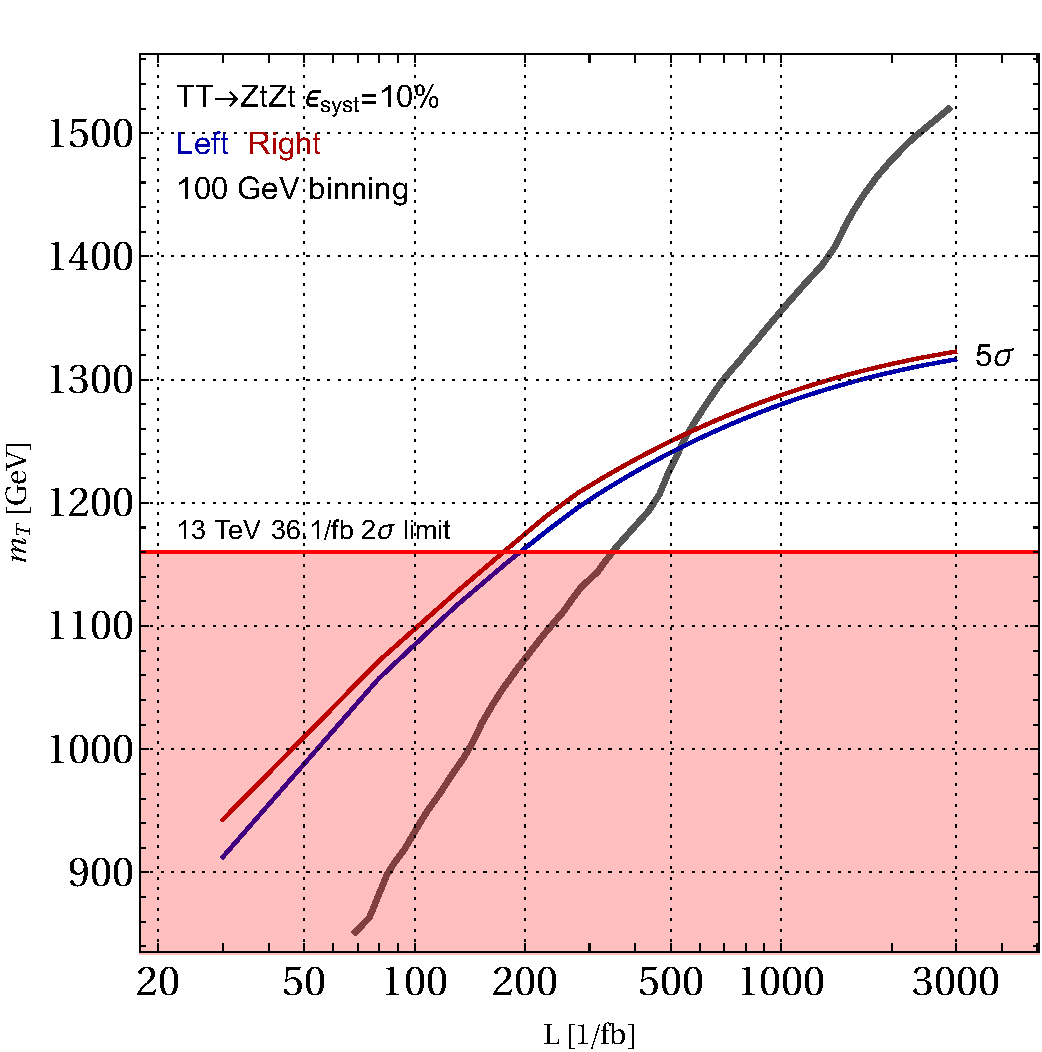
\includegraphics[width=0.45 \textwidth]{\main/section7OtherSignatures/img/discrimination_13TeV_10pc_100GeV_singlelep_ZtZt.pdf}
\caption{Projected 5$\sigma$ discovery (blue and red) and 2$\sigma$ discrimination (gray) reach of the ATLAS single lepton search~\cite{Aaboud:2017qpr} for a $T$ VLQ decaying with 100\% branching ratio into the $Zt$ final state. The blue and red lines correspond to the discovery reach for the left-handed and right-handed coupling structure assuming an uncertainty on the background determination of 10\%. The red shaded area correspond to the present experimental limit from for a VLQ decaying with 100\% branching ratio into the $Zt$ final state, namely 1160 GeV~\cite{Aaboud:2017qpr}\label{fig:13-discr}}
\end{center}
\end{figure}

The results are shown in \fig{fig:13-discr}, where we illustrate the 5$\sigma$ discovery reach for VLQs with left- or right-handed coupling together with the $2\sigma$ discrimination contour from the $\chi^2$ fit.
We see that if a VLQ with a mass lighter than 1200 GeV is discovered, a mild increase in integrated luminosity will be needed to disentangle the two hypotheses, while the collected dataset will already be enough for the discrimination if a VLQ heavier than 1200 GeV is found with a $5\sigma$ significance.

%\subsubsection{Discovery and discrimination at HE-LHC}
\paragraph*{Discovery and discrimination at HE-LHC}

The results obtained for the 13 TeV LHC show that with the signal region currently used in the ATLAS search we have considered, the LHC discovery reach will mildly increase when further data will be collected, due to the fact that at hadron colliders the contribution of the PDFs drops when the transferred momentum of the process approaches the kinematic limit $\sqrt{s}/2$.\footnote{Clearly an optimization of the signal regions can be performed to increase the sensitivity already at the current LHC energy.}
We then estimate here what is the mass reach of the high energy upgrade of the LHC for discovering pair-produced VLQs and discriminate their coupling structure.

\begin{figure}
\begin{center}
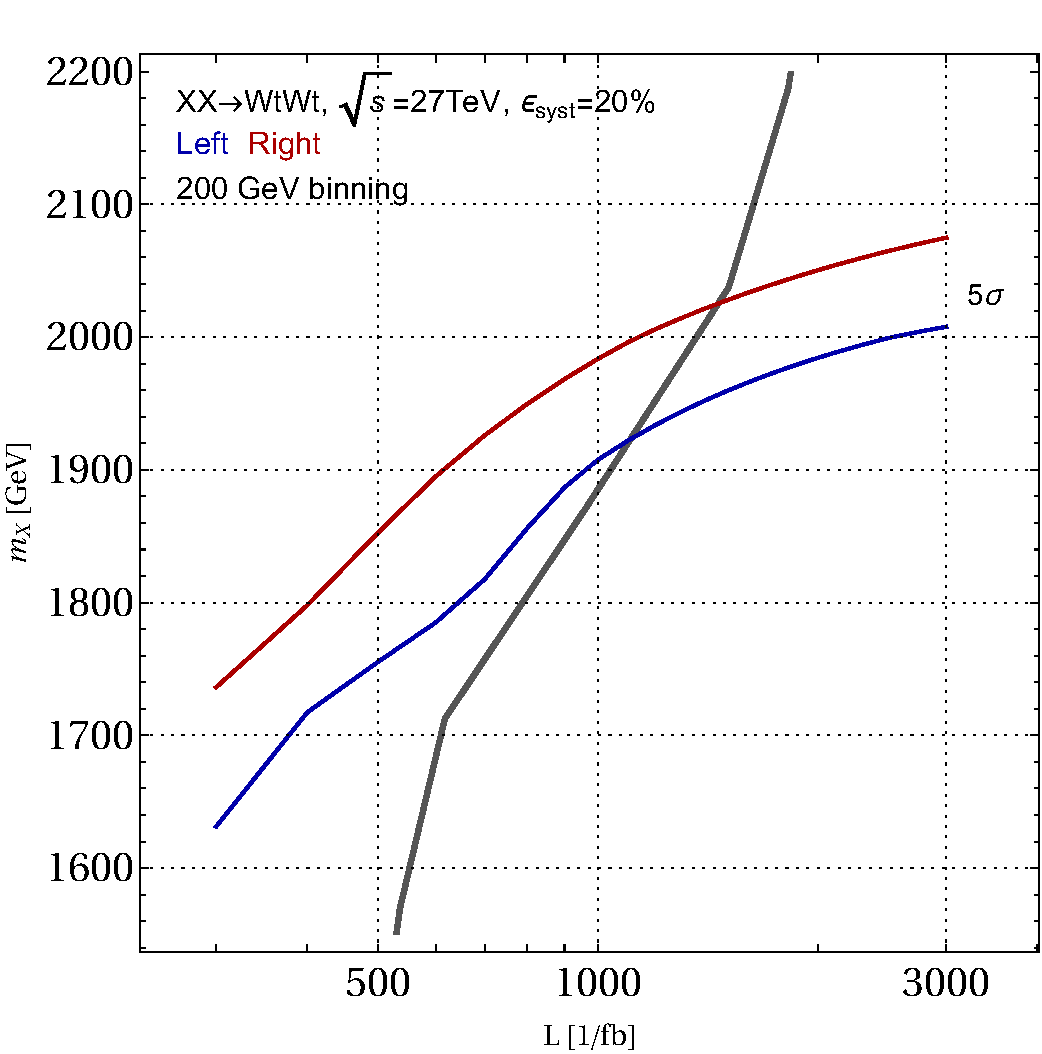
\includegraphics[width=0.45 \textwidth]{\main/section7OtherSignatures/img/27TeV_newcard.pdf}
\caption{Projected discovery (blue and red) and discrimination (gray)  reach of the 2SSL search for a $X$ VLQ decaying with 100\% branching ratio into the $Wt$ final state at $\sqrt{s}=27$ TeV. We use the $p_T$ distribution of the sub-leading lepton with a binning of 200 GeV and assume an uncertainty on the background determination of 20\%.\label{fig:33Lumi_2}}
\end{center}
\end{figure}

We focus on the case of a VLQ with charge 5/3 decaying into a $W$ boson and a top quark and closely follow the search strategy defined in \citeref{Avetisyan:2013rca}. In this case we consider for discrimination the $p_T$ distribution of the sub-leading lepton, which is almost always coming from the SM top decay. With the same statistical procedure adopted in the previous Section and rescaling the backgrounds yields given in \citeref{Avetisyan:2013rca} for $\sqrt{s}=33\;$TeV we show in \fig{fig:33Lumi_2} the results obtained for $\sqrt{s}=27\;$TeV. Our results show that a discrimination among the left- and right-handed coupling hypotheses is possible in all the discovery range accessible at a 27 TeV collider. In particular, if a VLQ with mass greater than $\sim 2000\;$GeV is discovered, the collected data set will already be sufficient to exclude one of the two coupling structure. 

%\subsubsection{Conclusion}
\paragraph*{Conclusion}

Our study shows that if a VLQ interacting with the SM top quark is observed in the high-luminosity phase of the LHC or in high-energy future upgrades, it will be possible to exploit the kinematic properties of its decay products for discriminating the dominant chirality of its couplings. 
We have performed a $\chi^2$ analysis to discriminate the $p_T$ distributions of the leading lepton for the pair production process of a left- or right-handed VLQ with charge 2/3 decaying to $Z$ and top, considering a single-lepton signal region used in a search from ATLAS at 13 TeV and projecting the results for the HL-LHC phase. Subsequently, we have used the same analysis technique considering the $p_T$ distributions of the sub-leading lepton, for a VLQ with charge 5/3 decaying to $W$ and top observed in a HE-LHC upgrade at 33 TeV considering a same-sign dilepton signal region. In both cases we find that a 2$\sigma$ discrimination is possible within the discovery range of the machines.


